\section{Задание №5}

\begin{enumerate}
        \item Пусть $X \sim \mbox{N}(\mu,\,\sigma^2)$. Убедиться в справедливости ЗБЧ и ЦПТ, то есть исследовать поведение суммы $S_n$ и эмперического распределения случайной величины
$$
        \sqrt{n}
        \left(
                \frac{S_n}{n} - \mu
        \right).
$$
        \item Считая $\mu$ и $\sigma$ неизвестными, для пункта 1 построить доверительные интервалы для среднего и дисперсии.
        \item Пусть $X \sim \mbox{C}(a,\,b)$ имеет распределение Коши со сдвигом $a$ и масштабом $b$. Проверить эмперически, как ведут себя суммы $\frac{S_n}{n}$. Результат объяснить, а также найти закон распределения данных сумм.
\end{enumerate}


\subsection{Закон больших чисел. Центральная предельная теорема.}

\begin{theorem}[Закон больших чисел]
        Пусть $X_1,\,X_2,\,\ldots,\,X_n,\,\ldots$ ---  последовательность независимых одинаково распределенных случайных величин, определенных на одном вероятностном пространстве $(\Omega,\, \mathcal{F},\, \p)$, с конечным превым моментом, равным $\E\,X_i = \mu$. Обозначим за $S_n = \sum_{i = 1}^{n} X_i$. Тогда
$$
        \frac{S_n}{n} \xrightarrow{\p} \mu,
$$
то есть
$$
        \forall \varepsilon > 0
        \quad
        \lim\limits_{n\to\infty}
        \p\left(\,
        \left|
                \frac{S_n}{n} - \mu
        \right|
        < \varepsilon
        \right)
        = 1.
$$
\end{theorem}

\begin{theorem} [Центральная предельная теорема]
        Пусть $X_1,\,X_2,\,\ldots,\,X_n,\,\ldots$ ---  последовательность независимых одинаково распределенных случайных величин, определенных на одном вероятностном пространстве $(\Omega,\, \mathcal{F},\, \p)$, с конечным превым моментом, равным $\E\,X_i = \mu$ и конечной дисперсией $\Var\,X_i = \sigma^2 \neq 0$. Обозначим за $Y_n = \frac{S_n - \mu n}{\sigma \sqrt{n}}$, тогда
$$
        Y_n \xrightarrow{dist.} \mbox{N}(0,\,1),
$$
то есть
$$
        \lim\limits_{n\to\infty}\p(Y_n < x) =
        \frac{1}{\sqrt{2\pi}}\int\limits_{-\infty}^{x} e^{-\frac{t^2}{2}}\,dt
        = F_N(x).
$$
\end{theorem}


\subsection{Построение доверительных интервалов для среднего и дисперсии нормальной случайной величины.}

Пусть теперь $X_1,\,X_2,\,\ldots,\,X_n$ ---  независимая выборка из некоторого нормального распределения $\mbox{N}(\mu,\,\sigma^2)$ с неизвестными параметрами. Построим доверительный интервал для неизвестного среднего.

\begin{theorem}
        Случайная величина
$$
        T = \sqrt{n} \cdot \frac{\overline X - \mu}{s},
$$
        где $\overline X$ --- выборочное среднее, а $s$ --- несмещенное выборочное стандартное отклонение, имеет распределение Стьюдента с $(n-1)$ степенью свободы.
\end{theorem}

Обозначим за $t_{\alpha}$ квантиль распределения Стьюдента с $(n-1)$ степенью свободы порядка $\alpha$. В силу симметрии данного распределения имеем, что
$$
        \p(-t_{1 - \nicefrac{\alpha}{2}} \leqslant T \leqslant t_{1 - \nicefrac{\alpha}{2}}) = 1 - \alpha,
$$
$$\Downarrow$$
$$
        \p(\overline X - \frac{s}{\sqrt{n}} t_{1 - \nicefrac{\alpha}{2}} \leqslant \mu \leqslant \overline X + \frac{s}{\sqrt{n}} t_{1 - \nicefrac{\alpha}{2}})
        =
        1 - \alpha.
$$
Таким образом мы получили доверительный интервал для математического ожидания~$\mu$:
$$
        \overline X - \frac{s}{\sqrt{n}} t_{1 - \nicefrac{\alpha}{2}} \leqslant \mu \leqslant \overline X + \frac{s}{\sqrt{n}} t_{1 - \nicefrac{\alpha}{2}},
$$
длина которого равна
$$
L(n) = 2\frac{s}{\sqrt{n}}\,t_{1 - \nicefrac{\alpha}{2}} = O(n^{-\nicefrac{1}{2}}) \xrightarrow[n\to\infty]{} 0.
$$

Теперь будем строить доверительный интервал для дисперсии. В этом нам поможет теорема Фишера для нормальных выборок.

\begin{theorem}[Фишер]
        Случайная величина
$$
        H = \frac{s^2}{\sigma^2}(n - 1)
$$
        имеет распределение хи-квадрат с $(n-1)$ степенью свободы.
\end{theorem}

Обозначим за $\chi^2_{\alpha}$ квантиль распределения хи-квадрат с $(n-1)$ степенью свободы порядка $\alpha$. Аналогично предыдущим рассуждениям имеем:
$$
        \p\left(\chi^2_{\frac{1 + \alpha}{2}} \leqslant H \leqslant \chi^2_{\frac{1 - \alpha}{2}}\right) = \alpha,
$$
$$
        \Downarrow
$$
$$
        \p\left(
                \frac{s^2}{\chi^2_{\frac{1 + \alpha}{2}}}
                (n - 1)
                \leqslant
                \sigma^2
                \leqslant
                \frac{s^2}{\chi^2_{\frac{1 - \alpha}{2}}}
                (n - 1)
        \right) = \alpha.
$$
Таким образом мы получили доверительный интервал для дисперсии
$$
        \frac{s^2}{\chi^2_{\frac{1 + \alpha}{2}}}
        (n - 1)
        \leqslant
        \sigma^2
        \leqslant
        \frac{s^2}{\chi^2_{\frac{1 - \alpha}{2}}}
        (n - 1),
$$
длина которого равна
$$
        L(n) = s^2 (n - 1) \left(
                \frac{s^2}{\chi^2_{\frac{1 - \alpha}{2}}}
                -
                \frac{s^2}{\chi^2_{\frac{1 + \alpha}{2}}}
        \right) \xrightarrow[n\to\infty]{} 0.
$$


\subsection{Поведение частичных сумм распределения Коши}

Рассмотрим случайную величину $X \sim \mbox{C}(a,\,b)$. Эмпирически можно увидеть, что выборка таких случайных величин не удовлетворяет закону больших чисел. Разберемся почему это так.

\begin{definition}
        Пусть $\xi$ --- произвольная случайная величина, определенная на вероятностном пространстве $(\Omega,\, \mathcal{F}, \p)$. Тогда ее \textit{математическим ожиданием} называется
$$
        \E\,\xi = \int\limits_{\Omega}\xi(w)\p(dw).
$$
\end{definition}

Получается, что, так как значение
$$
        \E\,X =
        \frac{b}{\pi}
        \int\limits_{-\infty}^{+\infty} \frac{1}{(x - a)^2 + b^2}\,dx
$$
не определено, то не выполняется одно из условий закона больших чисел. Как же ведут себя частичные суммы распределения Коши? На этот вопрос можно ответить при помощи следующего утверждения.

\begin{assertion}[Свойство устойчивости]
        Пусть $X_1,\,X_2,\,\ldots,\,X_n,\,\ldots$ --- независимые одинаково распределенные случайные величины, имеющие распределение Коши с параметрами $a$ и $b$. Тогда случайная величина
$$
        S_n = \frac 1 n \sum_{k = 1}^n X_k
$$
        также имеет распределение Коши с параметрами $a$ и $b$, причем для любого $n$.
\end{assertion}

\begin{proof}
        Воспользуемся аппаратом характеристических функций. Известно, что характеристическая функция случайной величины $X\sim\mbox{C}(a,\,b)$ имеет вид
$$
        \varphi_X(x) = e^{aix - b|x|}.
$$
        Вспомним следующие свойства характеристических функций:
$$
        \varphi_{aX}(x) = \varphi_X(ax),
$$
$$
        \varphi_{\sum_{k = 1}^{n}X_k}(x) = \prod_{k = 1}^{n} \varphi_{X_k}(x).
$$
Теперь мы можем легко найти характеристическую функцию случайной величины $S_n$:
$$
        \varphi_{S_n}(x)
        =
        \varphi_{\sum_{k = 1}^{n}X_k}(\nicefrac{x}{n})
        =
        \prod_{i = 1}^n \varphi_{X_k}(\nicefrac{x}{n})
        =
        \left(
                \varphi_{X_1}(\nicefrac{x}{n})
        \right)^n
        =
        \left(
                e^{\frac{aix}{n} - \left|\frac{x}{n}\right|b}
        \right)^n
        =
        e^{aix - b|x|}
        =
        \varphi_{X_1}(x).
$$
Так как характеристические функции $S_n$ и $X_k$ совпадают, то их распределения тоже совпадают. Утверждение доказано.
\end{proof}

\clearpage
\begin{figure}[t]
        \noindent
        \centering
        {
                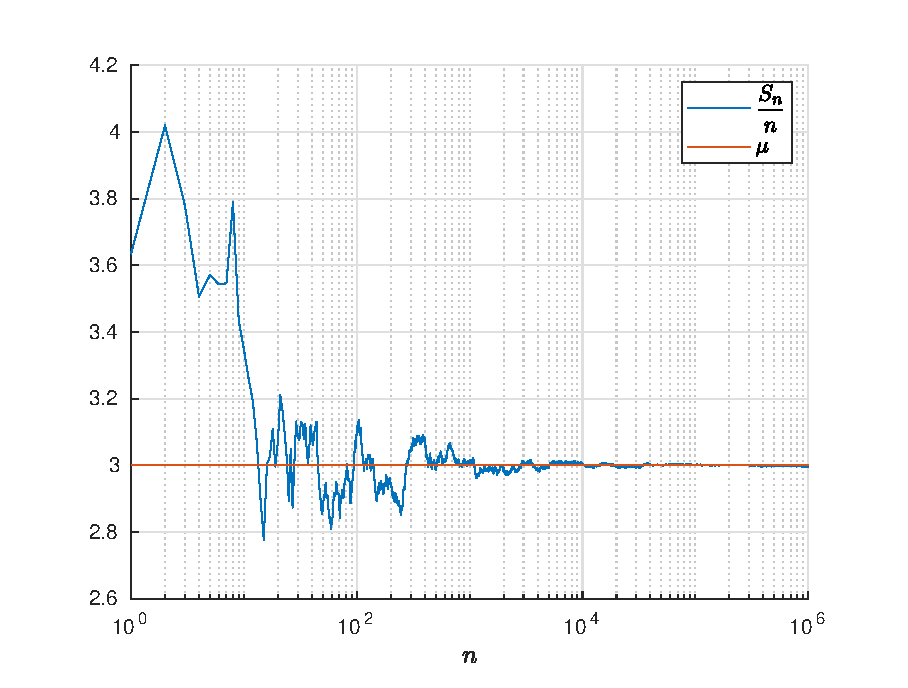
\includegraphics[width=120mm]{task_05/zbc.eps}
        }
        \caption{Иллюстрация выполнения закона больших чисел для нормально распределенной случайной величины с параметрами $\mu = 3$, $\sigma^2 = 4$.}
\end{figure}
\begin{figure}[b]
        \noindent
        \centering
        {
                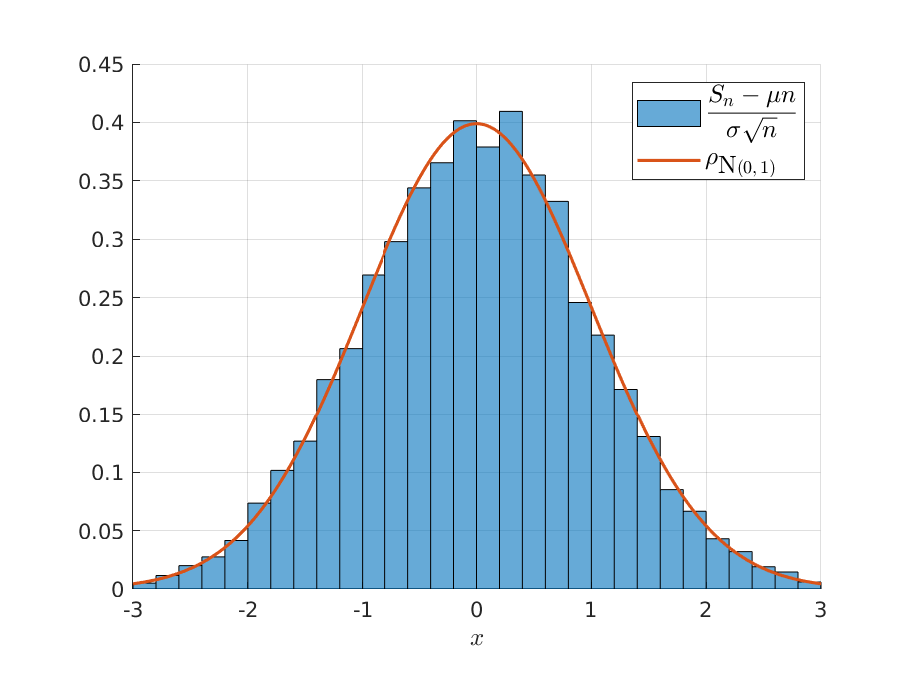
\includegraphics[width=120mm]{task_05/cpt10000-10000.eps}
        }
        \caption{Иллюстрация выполнения центральной предельной теоремы для нормально распределенной случайной величины с параметрами $\mu = 3$, $\sigma^2 = 4$. Было проведено $10^4$ испытаний по генерации $S_n$, где $n = 10^4$.}
\end{figure}
\begin{figure}[t]
        \noindent
        \centering
        {
                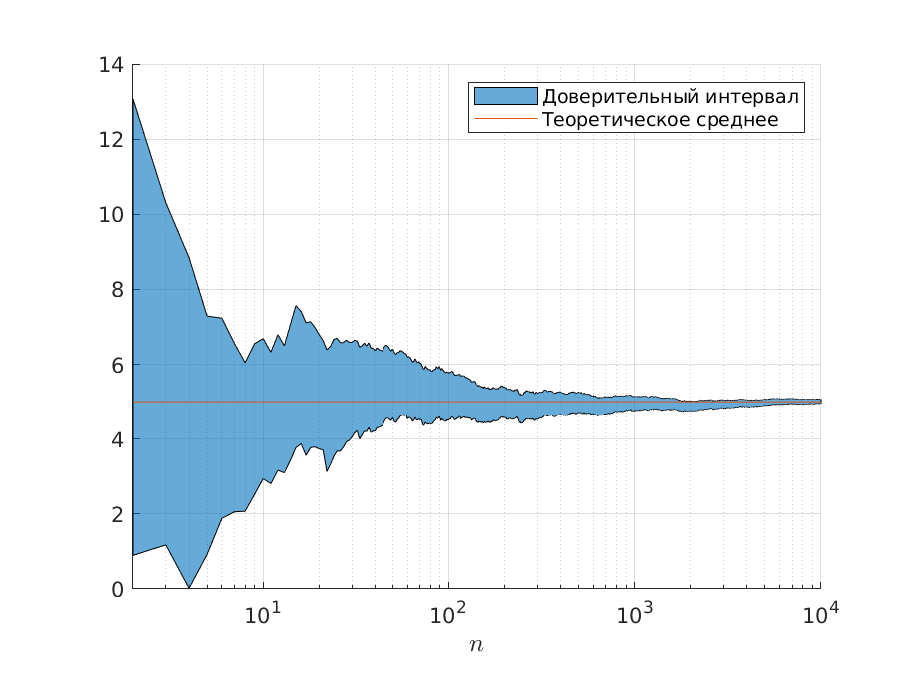
\includegraphics[width=120mm]{task_05/mu-interval.eps}
        }
        \caption{Доверительный интервал для математического ожидания случайной величины нормального распределения с параметрами $\mu = 5$, $\sigma^2 = 9$.}
\end{figure}
\begin{figure}[b]
        \noindent
        \centering
        {
                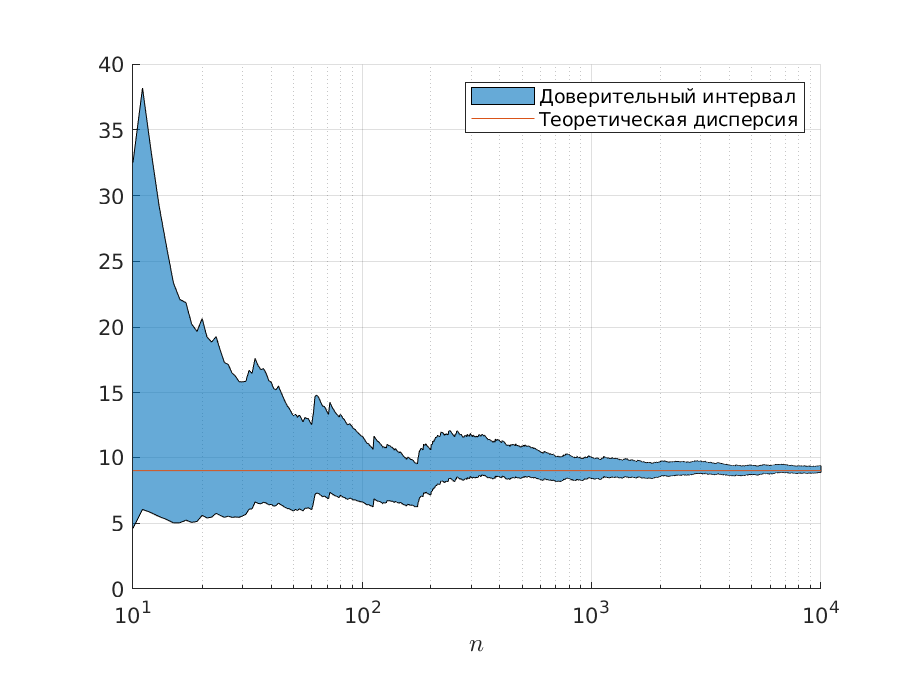
\includegraphics[width=120mm]{task_05/sigma-interval.eps}
        }
        \caption{Доверительный интервал для дисперсии случайной величины нормального распределения с параметрами $\mu = 5$, $\sigma^2 = 9$.}
\end{figure}
\begin{figure}[t]
        \noindent
        \centering
        {
                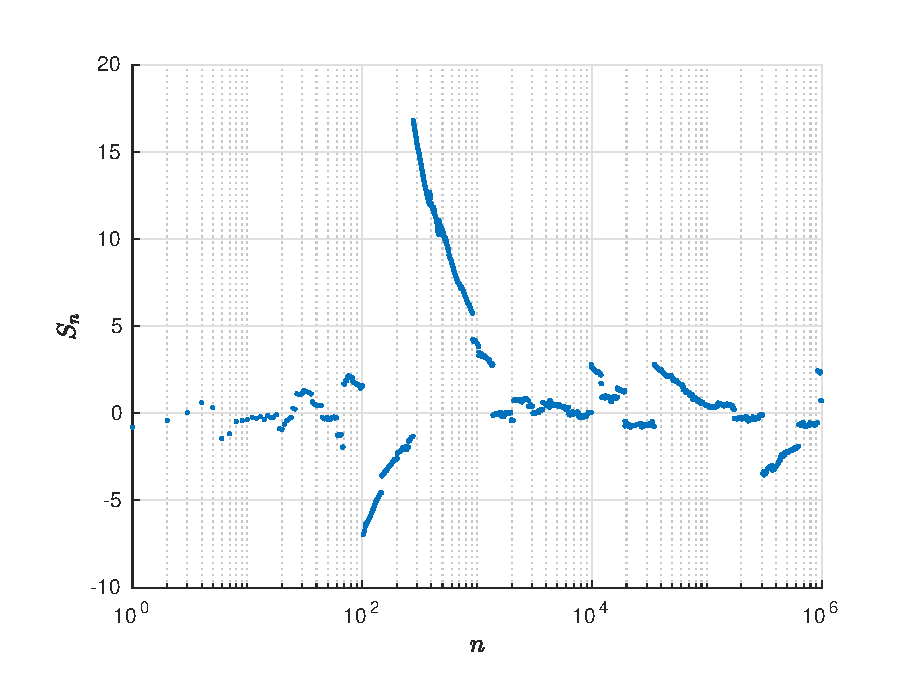
\includegraphics[width=120mm]{task_05/cauchy-zbc.eps}
        }
        \caption{Иллюстрация неприменимости закона больших чисел к распределению Коши. Поведение частичных сумм случайной величины Коши с параметрами $a = 0$, $b = 1,5$.}
\end{figure}
\begin{figure}[b]
        \noindent
        \centering
        {
                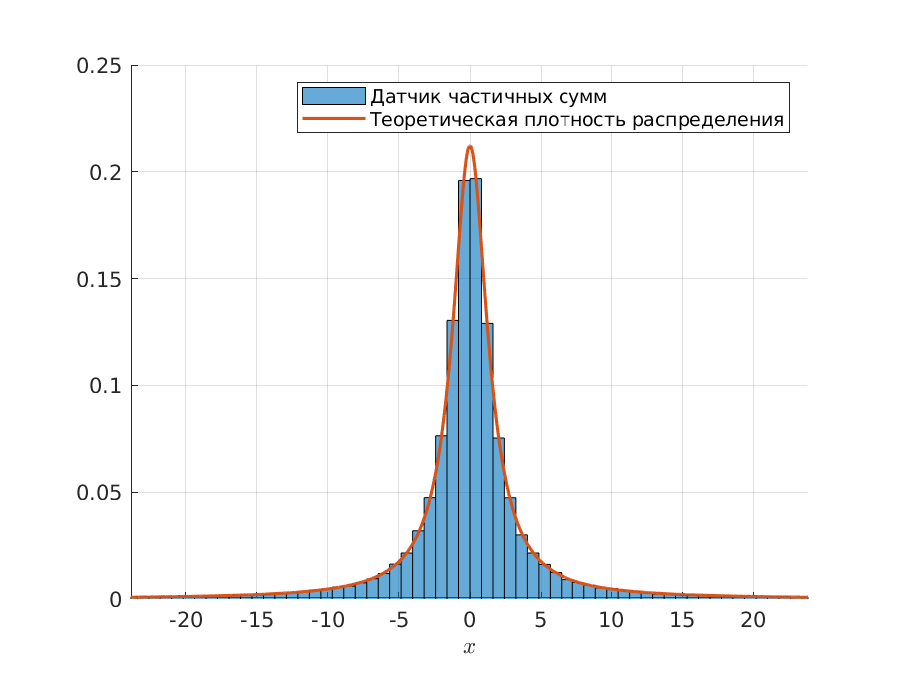
\includegraphics[width=120mm]{task_05/cauchy0-1d5-100-100000.eps}
        }
        \caption{Иллюстрация свойства устойчивости распределения Коши. Представлена гистограмма распределения частичных сумм $S_{100}$ случайной величины Коши с параметрами $a = 0$, $b = 1,5$. Объем выборки --- $10^5$.}
\end{figure}